% Remplacement local des encadrés de placeholders du chapitre FeastVerse par
% les illustrations réelles. Ce fichier est chargé dans un groupe LaTeX dédié
% au chapitre FeastVerse afin de ne pas modifier le comportement de \fbox
% dans le reste du dossier.
\newcounter{feastversefigureplaceholder}
\setcounter{feastversefigureplaceholder}{0}

\renewcommand{\fbox}[1]{%
  \stepcounter{feastversefigureplaceholder}%
  \ifcase\value{feastversefigureplaceholder}%
  \or
    % Architecture générale de l'API.
    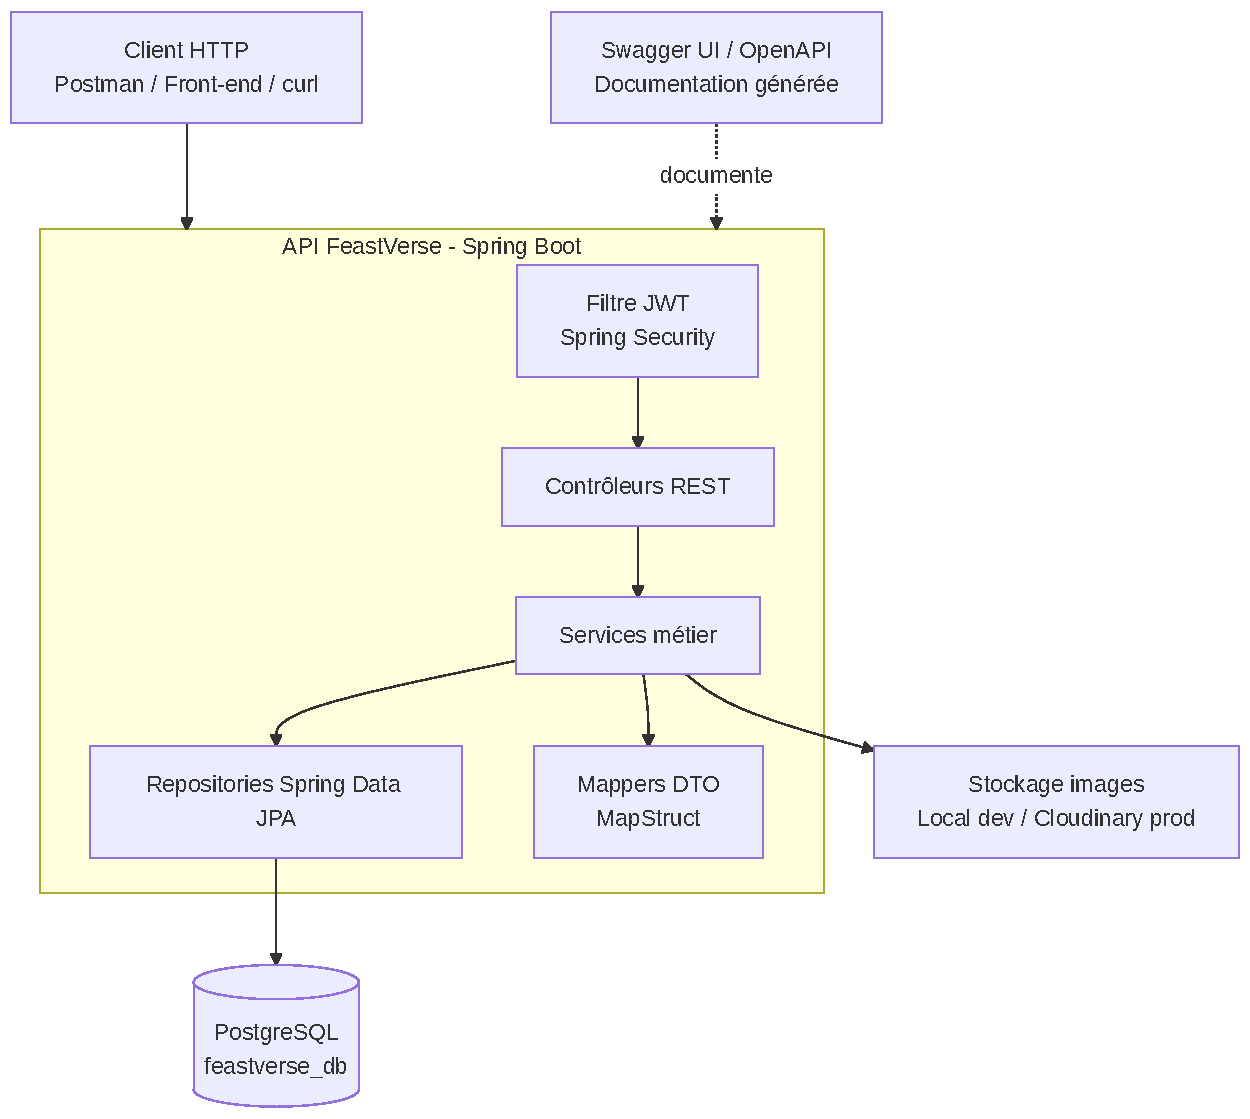
\includegraphics[width=0.92\textwidth,height=0.48\textheight,keepaspectratio]{figures/feastverse/archi2.pdf}%
  \or
    % Recherche, pagination et filtrage dans Swagger UI.
    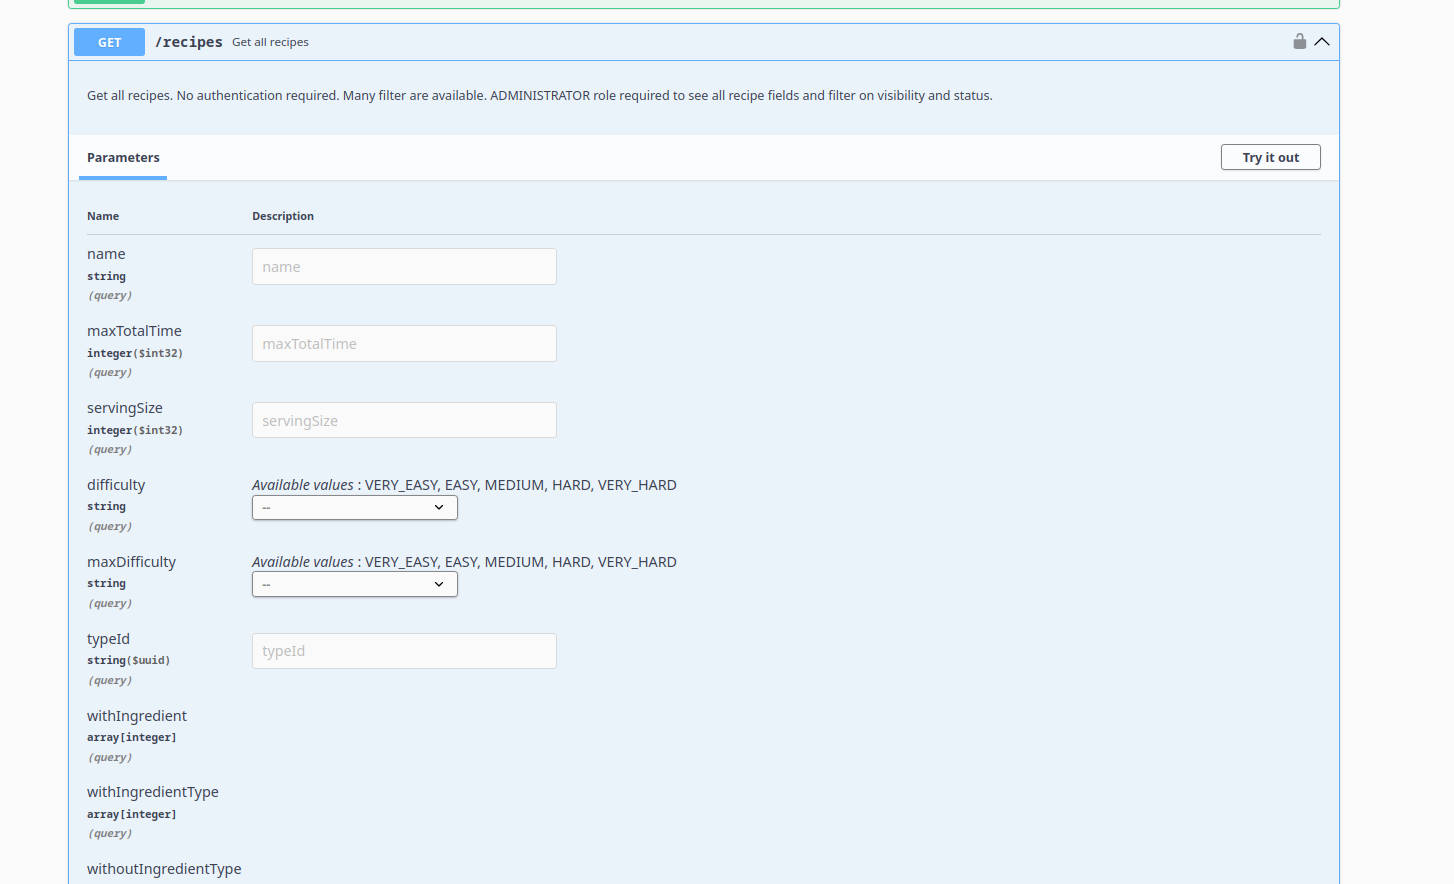
\includegraphics[width=\textwidth,height=0.48\textheight,keepaspectratio]{figures/feastverse/swagger.png}%
  \or
    % Requête Postman, notamment pour les données multipart et l'image.
    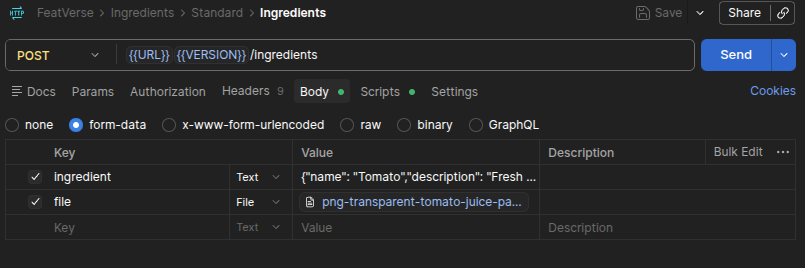
\includegraphics[width=\textwidth,height=0.32\textheight,keepaspectratio]{figures/feastverse/postman.png}%
  \or
    % Organisation de la collection Postman.
    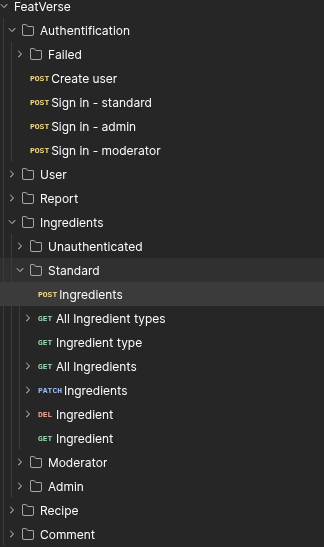
\includegraphics[width=0.52\textwidth,height=0.50\textheight,keepaspectratio]{figures/feastverse/postman_folder.png}%
  \or
    % Détail d'un endpoint documenté dans Swagger/OpenAPI.
    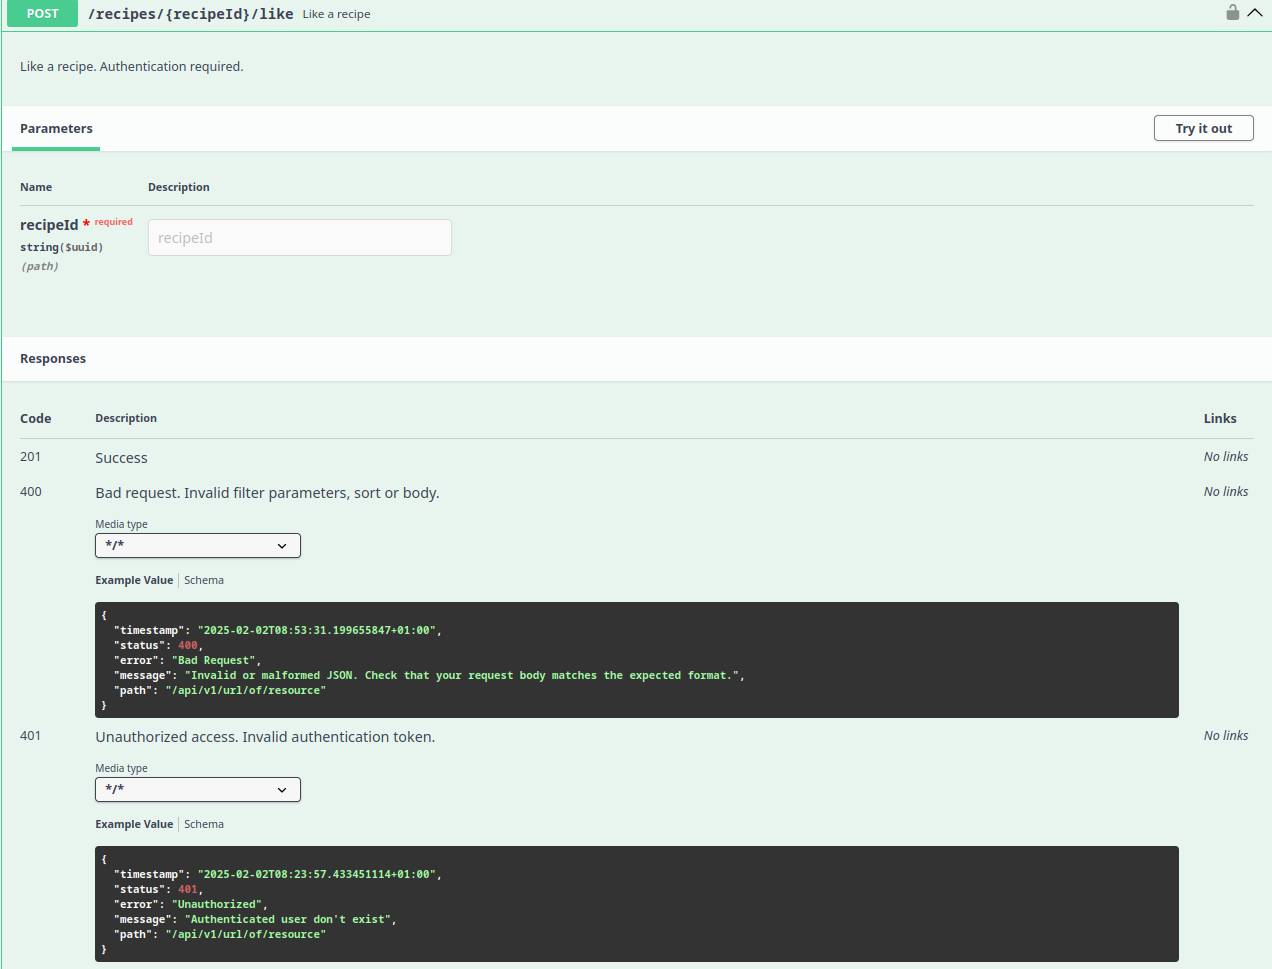
\includegraphics[width=\textwidth,height=0.52\textheight,keepaspectratio]{figures/feastverse/swagger_endpoint_documente.png}%
  \or
    % Site de documentation MkDocs.
    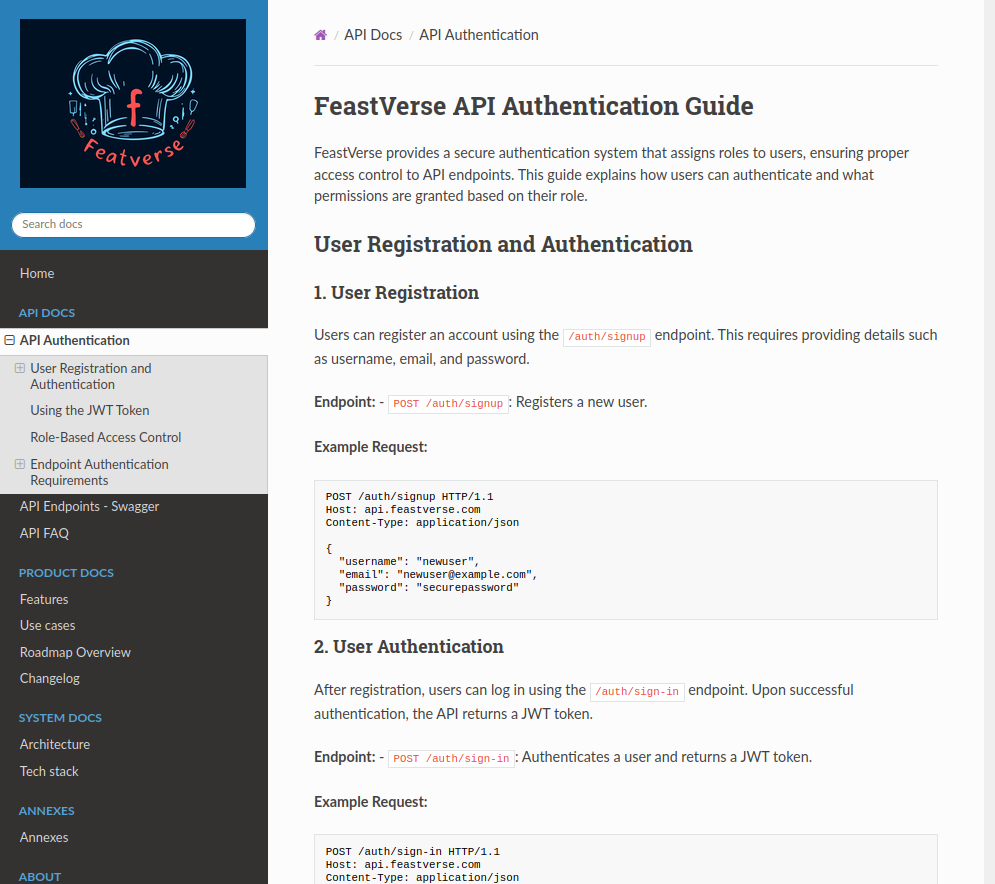
\includegraphics[width=0.92\textwidth,height=0.52\textheight,keepaspectratio]{figures/feastverse/documentation_mkdocs.png}%
  \or
    % L'historique Railway n'est plus disponible : ne pas fabriquer de
    % capture. La configuration de production et le fonctionnement du
    % déploiement sont décrits et justifiés dans le texte du chapitre.
    \begin{minipage}{0.88\textwidth}
      \centering
      \small\itshape
      L'historique visuel des déploiements Railway n'est plus disponible.\\[0.15cm]
      Le déploiement est donc étayé par la configuration de production,
      la séparation des variables d'environnement et la description du lien
      entre le dépôt GitHub et le service Railway, sans reconstituer une preuve
      graphique qui n'a pas été conservée.
    \end{minipage}%
  \else
    \PackageError{feastverse-figures}{Nombre de placeholders FeastVerse inattendu}{Le chapitre FeastVerse contient plus de 7 appels a \string\fbox.}%
  \fi
}
